
\documentclass{article}

%-------------------------------------------------------------------------------------------------------------
%  package
%--------------------------------------------------------------------------------------------------------------
%版面規劃(a4大小,上下左右距0.9inch)
\usepackage[a4paper,margin=0.8in]{geometry}
%和插入圖片相關的package
\usepackage{graphicx}
\usepackage[tight]{subfigure}
\subfiguretopcaptrue
\usepackage{amsmath,booktabs,threeparttable,url, bm}
%\usepackage[hyphenbreaks]{breakurl}
%連結註腳網頁
\usepackage[colorlinks,linkcolor=blue]{hyperref}
%中文化package
\usepackage{CJKutf8}

%\newcommand{\cntext}{\begin{CJK}{UTF8}{bsmi}\end{CJK}}

\title{Assignment 5 of Computational Astrophysics in NTHU}
\author{Wei-Hsiang Yu 游惟翔}


%-------------------------------------------------------------------------------------------------------------
%  文件開始
%--------------------------------------------------------------------------------------------------------------
\begin{document}

\begin{CJK}{UTF8}{bsmi}
%中文化需要加上此行才有title/author/date
\maketitle
\end{CJK}



%-------------------------------------------------------------------------------------------------------------
%  Programming Assignments
%--------------------------------------------------------------------------------------------------------------
\section{Programming Assignments}
%Q1---------------------------------------------------------------------
\textbf{Q1 : Solve $x^3+1.5x^2-5.75x+4.37$\\}

I first try to search \emph{Wolfram}
\footnote{Wolfram:\href{www.wolframalpha.com}{www.wolframalpha.com}}
to find out the approximately solution of this equation, the root is in range -3 and -4.(Fig.\ref{fig:1_1})
% %-------------------------------
\begin{figure}[h]
    \centering 
	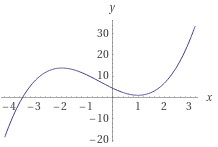
\includegraphics[scale=0.75]{pro1.jpg}
	\caption{The prediction of \emph{Wolfram}}%圖片註解
	\label{fig:1_1} %label 用這個就可以引用文章當中
\end{figure}
% %-------------------------------

In Fig.\ref{fig:1_2} we can see Newton's method has the fastest performance of those methods.  But if we given a wider range (as Fig.\ref{fig:1_3} of 0 to -4), Newton's method will first go to the right side and has poorer performance.(because the concavity is down and tendency is to right) So we can say that: if we can first know the tendency of solution, the Newton's and secant method will be better, but if we don't, they may won't be the best choice.


% %-------------------------------
\begin{figure}[h]
    \centering
    \subfigure[Convergence solution]{
        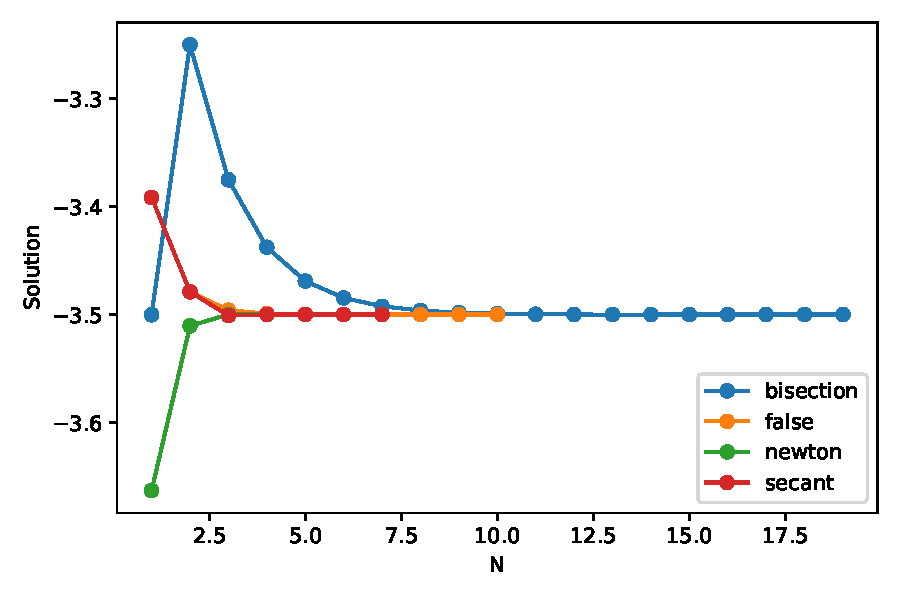
\includegraphics[scale=0.35]{fig_convergence_solution.pdf}
        \label{fig:1_2.1}
    }
    \subfigure[Convergence error]{
        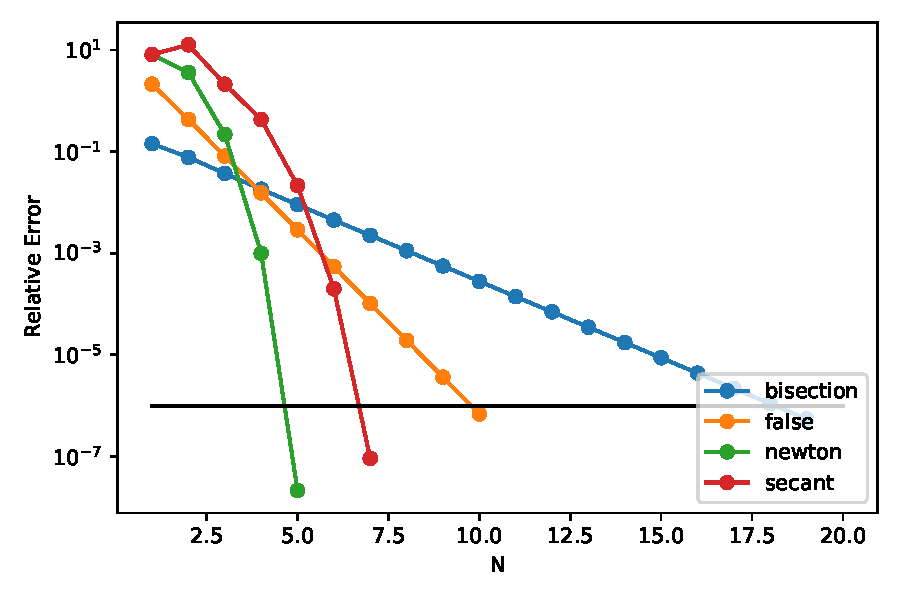
\includegraphics[scale=0.35]{fig_convergence_error.pdf}
        \label{fig:1_2.2} 
    }
    \subfigure[Convergence rate]{
        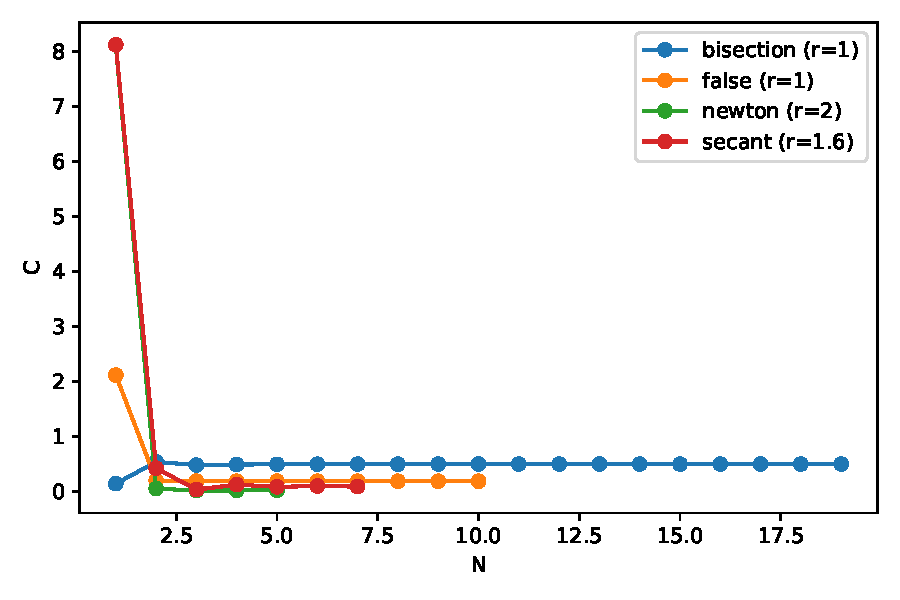
\includegraphics[scale=0.35]{fig_convergence_rate.pdf}
        \label{fig:1_2.3} 
    }
     \caption{Compared the performance of given a closer($-3\ -4$) range of initial value}
    \label{fig:1_2}
\end{figure}
% %-------------------------------
    
% %-------------------------------
\begin{figure}[h]
    \centering
    \subfigure[Convergence solution]{
        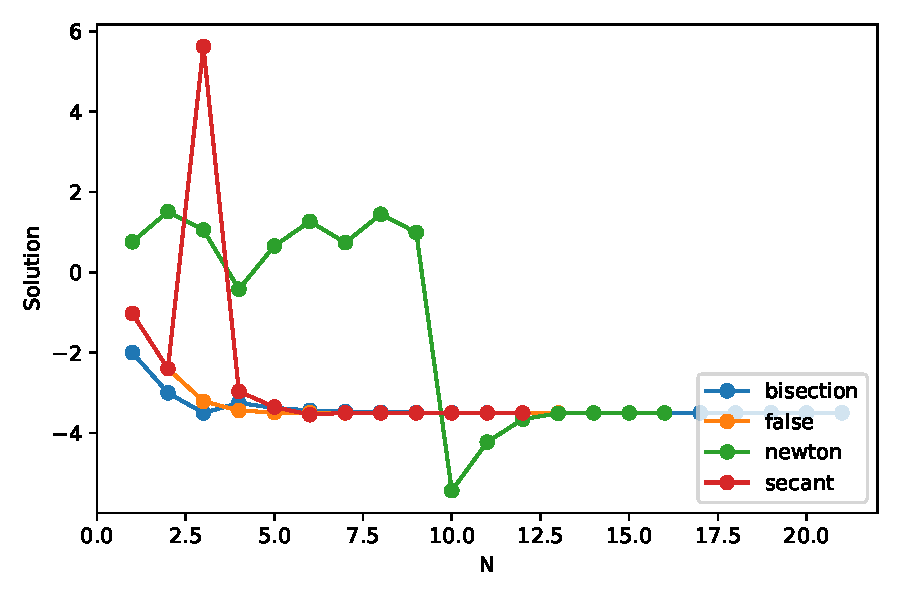
\includegraphics[scale=0.35]{fig_convergence_solution1.pdf}
        \label{fig:1_3.1}
    }
    \subfigure[Convergence error]{
        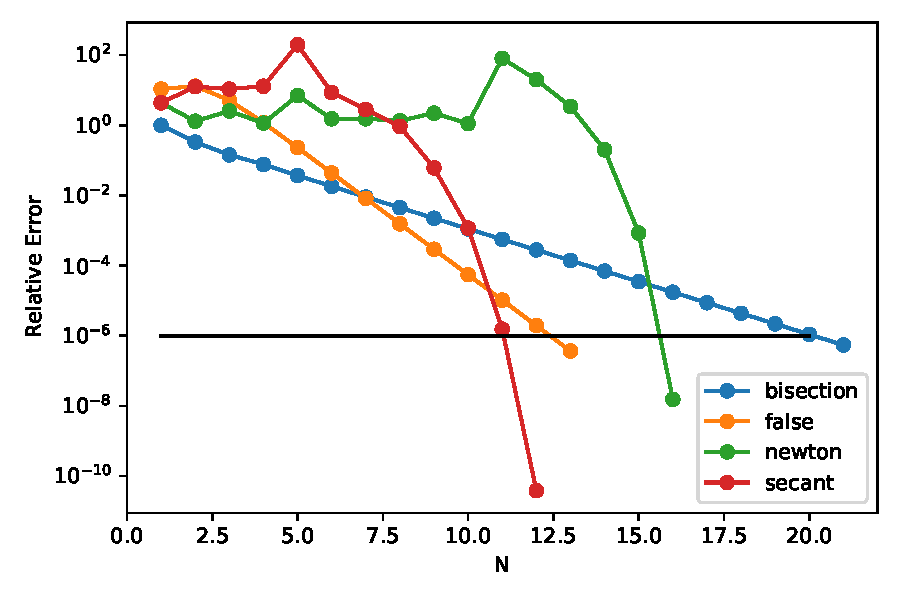
\includegraphics[scale=0.35]{fig_convergence_error1.pdf}
        \label{fig:1_3.2} 
    }
    \subfigure[Convergence rate]{
        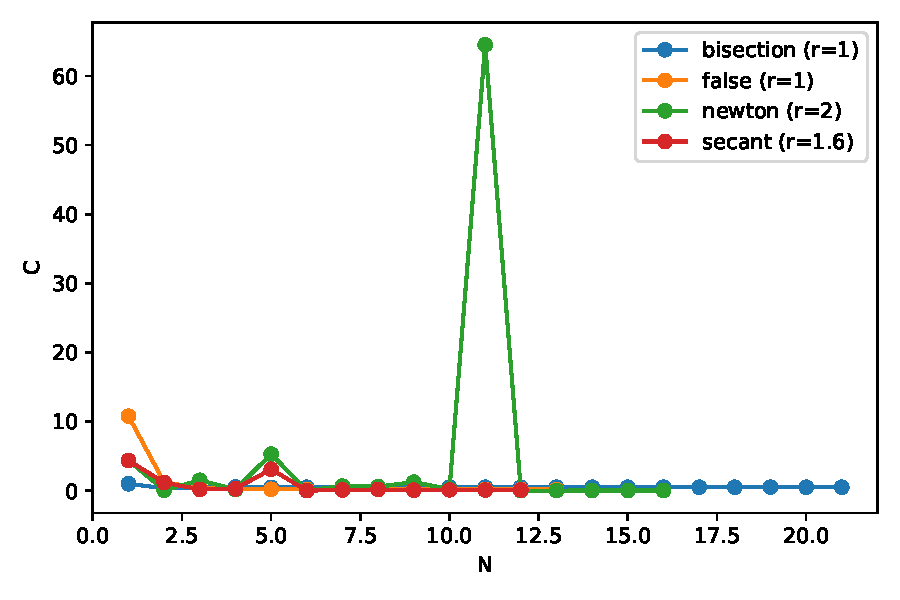
\includegraphics[scale=0.35]{fig_convergence_rate1.pdf}
        \label{fig:1_3.3} 
    }
    \caption{Compared the performance of given a wider($0\ -4$) range of initial value}
    \label{fig:1_3}
\end{figure}
% %-------------------------------
\underline{\textbf{Q2 : Doing the open integral}}
\begin{equation}
    I=\int_0^\infty \frac{1}{x^4+x^2+1}dx
    \label{eq:2-question}
\end{equation}

Now we can decompose the Eq.\ref{eq:2-question} into a simple form to do integral:

\begin{equation}
\frac{1}{x^4+x^2+1}=
\frac{1}{(x^2+x+1)(x^2-x+1)}=
\frac{1}{2}\frac{(x+1)}{(x^2+x+1)}-\frac{1}{2}\frac{(x-1)}{(x^2-x+1)}
\label{eq:2-part}
\end{equation}

$$
=\frac{1}{4}\frac{(2x+1)}{(x^2+x+1)}-\frac{1}{4}\frac{(2x-1)}{(x^2-x+1)}
+\frac{1}{4}\frac{1}{(x^2+x+1)}-\frac{1}{4}\frac{-1}{(x^2-x+1)}
$$

So we can integral the front two elements as \textbf{ln}; the last two elements as \textbf{atan}.

$$
\int \frac{1}{4}\frac{(2x+1)}{(x^2+x+1)}dx-\int\frac{1}{4}\frac{(2x-1)}{(x^2-x+1)}dx
+\int \frac{1}{4}\frac{1}{(x^2+x+1)}dx+\int \frac{1}{4}\frac{1}{(x^2-x+1)}dx
$$

$$
=\frac{1}{4}ln\begin{vmatrix}x^2+x+1\end{vmatrix}
-\frac{1}{4}ln\begin{vmatrix}x^2-x+1\end{vmatrix}
+\frac{1}{4} \int \frac{1}{{(x+\frac{1}{2})}^2+(\frac{\sqrt{3}}{2})^2} dx
+\frac{1}{4} \int \frac{1}{{(x-\frac{1}{2})}^2+(\frac{\sqrt{3}}{2})^2} dx
+c
$$

$$
=\frac{1}{4}ln\begin{vmatrix}x^2+x+1\end{vmatrix}
-\frac{1}{4}ln\begin{vmatrix}x^2-x+1\end{vmatrix}
+\frac{1}{2\sqrt{3}}tan^{-1}(\frac{2x+1}{\sqrt{3}})
+\frac{1}{2\sqrt{3}}tan^{-1}(\frac{2x-1}{\sqrt{3}})
+c
$$

\begin{equation}
I_{finite}
=
\int \frac{1}{x^4+x^2+1}dx
=
\frac{1}{4}ln
\begin{vmatrix}
\frac{x^2+x+1}{x^2-x+1}
\end{vmatrix}
+
\frac{1}{2\sqrt{3}}tan^{-1}(\frac{\sqrt{3}x}{1-x^2})
+c
\label{eq:2-finity}
\end{equation}

I divide the Eq.\ref{eq:2-question} into two parts with 2, so integral become 0$\sim$2 \& 2$\sim \infty$:

% %-------------------------------
\begin{figure}[h]
    \centering 
	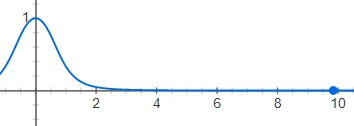
\includegraphics[scale=0.55]{pro2-1.jpg}
	\caption{The shape of $\frac{1}{x^4+x^2+1}$ }
	\label{fig:2-1} %label 用這個就可以引用文章當中
\end{figure}
% %-------------------------------

The first part is closed interval, so the value can be easily calculated (see Fig.\ref{fig:2-1}), I used the Simpson's rule to do integral, and get the result 0.8713...

\begin{equation}
\mbox{Simpson's rule}
\int_{a}^{b}f(x)dx\sim \frac{(b-a)}{6}(f(a)+4f(\frac{a+b}{2})+f(b))
\end{equation}

But the second part need to use the Eq.\ref{eq:2-finity} to do calculation.

$$ x \rightarrow  \infty,\quad ln\frac{\infty}{\infty} \rightarrow 0;\quad atan\frac{1}{-\infty}\rightarrow  0\quad \Rightarrow \quad I_{finite}\|_{\infty}\rightarrow  0$$

$$
\int_2^\infty \frac{1}{x^4+x^2+1}dx
=
I_{finite}\|_{\infty}-I_{finite}\|_{2}=-I_{finite}\|_{2}=0.03559
$$

% %-------------------------------
\begin{figure}[h]
    \centering 
	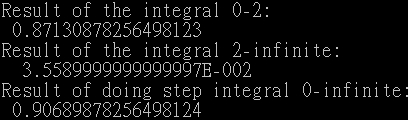
\includegraphics[scale=0.55]{pro2-2.jpg}
	\caption{The result of integral $\frac{1}{x^4+x^2+1}$ from 0 to $\infty$ }
	\label{fig:2-2} %label 用這個就可以引用文章當中
\end{figure}
% %-------------------------------


\underline{\textbf{Q3 : Stefan-Boltzmann constant}}

\textbf{3a.}
\begin{equation}
    \frac{\sigma _{B}T^{4}}{\pi}=\int_{0}^{\infty }B_{\nu}(T)d\upsilon
    \quad \mbox{where} \quad
    B_{\nu}(T)=\frac{2h\upsilon ^{3}}{c^{2}}\frac{1}{e^{\frac{h\upsilon }{KT}}-1}
    \label{eq:3-1}
\end{equation}

\begin{equation}
    \frac{\sigma _{B}T^{4}}{\pi}
    =
    \int_{0}^{\infty }\frac{2h\upsilon ^{3}}{c^{2}}\frac{1}{e^{\frac{h\upsilon }{KT}}-1}d\upsilon
    \label{eq:3-2}
\end{equation}

Then, we let $x\equiv \frac{h\upsilon }{kT}$, so $\upsilon =\frac{kT}{h}x$,
the differential of $\nu$ by $dx$ become $d\upsilon =\frac{kT}{h}dx$ and 
substitute it into Eq.\ref{eq:3-2}.

$$
\frac{\sigma _{B}T^{4}}{\pi}=\int_{0}^{\infty }\frac{2hk^3T^3}{h^3c^{2}}\frac{x^3}{e^x-1}\frac{kT}{h}dx 
$$

\begin{equation}
    \Rightarrow
    \sigma _{B}=\int_{0}^{\infty }\frac{2{\pi}k^4}{h^3c^{2}}\frac{x^3}{e^x-1}dx
    \label{eq:3-3}
\end{equation}

So the main problem will be doing the integral of $\frac{x^{3}}{e^{x}-1}$.
Google give us the shape of the function.(Fig.\ref{fig:3a1})

% %-------------------------------
\begin{figure}[h]
    \centering 
	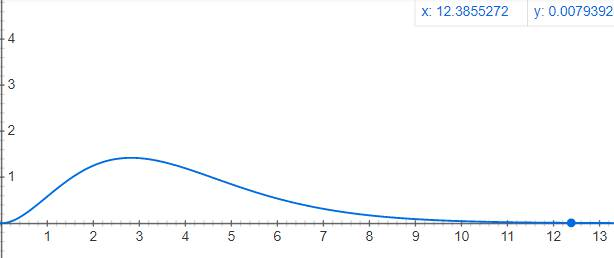
\includegraphics[scale=0.35]{pro3a.jpg}
	\caption{The shape of $\frac{x^{3}}{e^{x}-1}dx$}
	\label{fig:3a1} %label 用這個就可以引用文章當中
\end{figure}
% %-------------------------------

 In my program(Fig.\ref{fig:3a2}), I make the boundary of MC integral in region : x[0-2] ; y[0-1000], and record the number of points which values are lower than the function $\frac{x^{3}}{e^{x}-1}$.

Set the number of $N=10^8$, and we know the Stefan-Boltzmann constant=$5.670367 \times10^{-8} kg s^{-3} K^{-4}$, the error of this program compare to the real constant value is 0.28\%.
% %-------------------------------
\begin{figure}[h]
    \centering
    \subfigure[program]{
        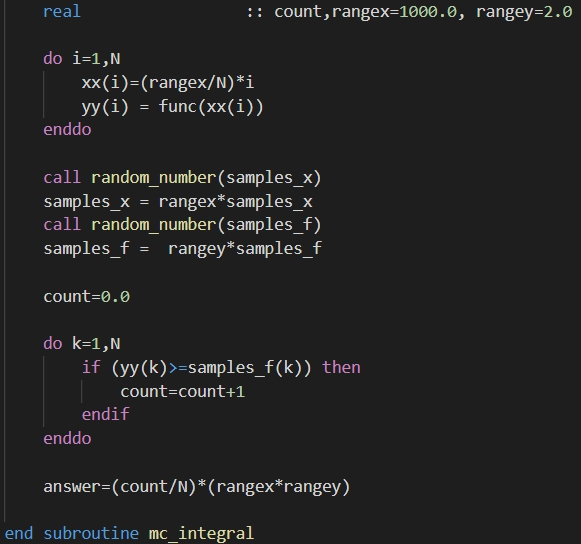
\includegraphics[scale=0.4]{pro3a-2.jpg}
        \label{fig:3a2-1}
    }
    \subfigure[result]{
        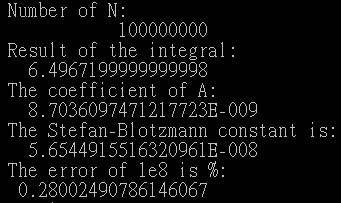
\includegraphics[scale=0.55]{pro3b8.jpg}
        \label{fig:3a2-2} 
    }
    \caption{The program and result  in fortran}
    \label{fig:3a2}
\end{figure}
% %-------------------------------

\textbf{3b.$\frac{1}{\sqrt{N}}$ law of MC integral}

Then, I try different numbers of N(from 1e8 to 1e3)(Fig.\ref{fig:3b2}.), and make a form in EXCEL to plot the relation(Fig.\ref{fig:3b1}.) between error and number of N.

The result of $\frac{1}{\sqrt{N}}$ and error is a highly positive correlation, the Pearson's r=0.9554, proof the $\frac{1}{\sqrt{N}}$ law.
% %-------------------------------
\begin{figure}[h]
    \centering
    \subfigure[N vs Error]{
        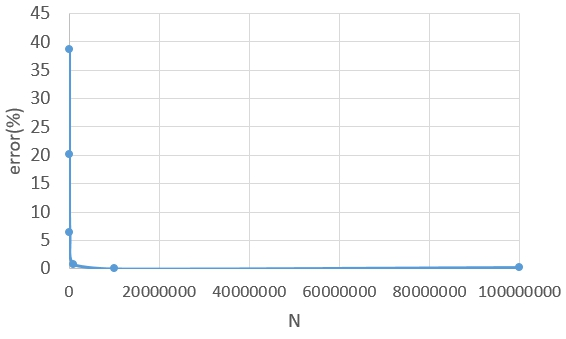
\includegraphics[scale=0.45]{pro3b1.jpg}
        \label{fig:3b-1}
    }
    \subfigure[$1/\sqrt{N}$ vs Error]{
        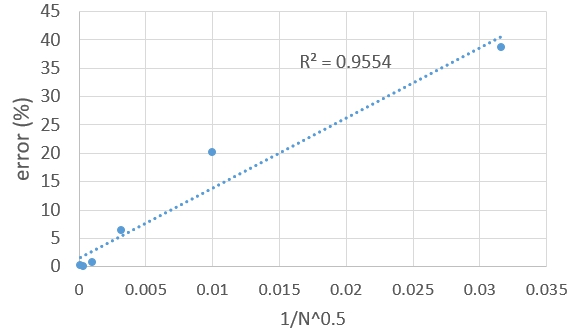
\includegraphics[scale=0.45]{pro3b2.jpg}
        \label{fig:3b-2} 
    }
    \caption{Compared the accuracy of given different number of N (Plot by  EXCEL)}
    \label{fig:3b1}
\end{figure}
% %-------------------------------

\underline{\textbf{Q4 : N-dimension of Newton's method}}

\begin{equation}
    f(x+s)~f(x)+J_f(x)s
\end{equation}

Where $J_f(x)$ is the Jacobian matrix of $f$ and 
$\{J_f(x)\}_{ij}=\frac{\partial f_i(x))}{\partial x_j}$, and if s satisfies the linear
system ${J_f(x)}s=-f(x)$, then x + s is taken as an approximate zero of f.

So we can say Jacobian matrix increase the dimensions of the original matrix but also make a nonlinear system become a linear system at the same time.

\begin{equation}
   f(x)=\begin{bmatrix}
    x_1+2x_2-2\\ 
    x_1^2+4x_x^2-4
    \end{bmatrix}
    =
    \begin{bmatrix}
    0\\ 
    0
    \end{bmatrix} 
    \label{eq:4-1}
\end{equation}


% %-------------------------------
\begin{figure}[h]
    \centering 
	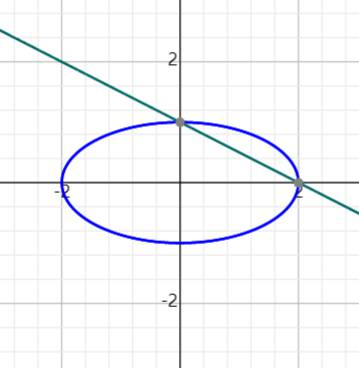
\includegraphics[scale=0.3]{pro4-1.jpg}
	\caption{The shape of Eq.\ref{eq:4-1}}
	\label{fig:4-1} %label 用這個就可以引用文章當中
\end{figure}
% %-------------------------------

Fig.\ref{fig:4-1} say there are two solutions in this nonlinear system, so I set the initial condition to (0,2)(Fig.\ref{fig:4-2.1}) \& (1,0)(Fig.\ref{fig:4-2.2}) to find the solutions (0,1) \& (2,0). Although the results still have some error, but the order of magnitude is small enough to ignore.(1e-17 to (0,1) \& 1e-18 to (2,0))

% %-------------------------------
\begin{figure}[h]
    \centering
    \subfigure[solution (0,1)]{
        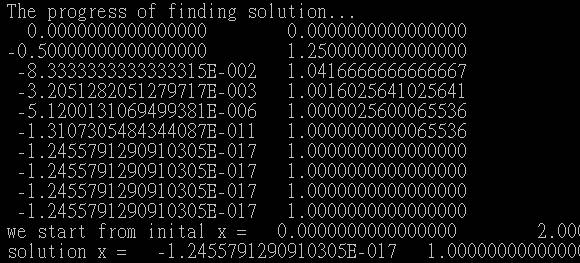
\includegraphics[scale=0.47]{pro4-2.jpg}
        \label{fig:4-2.1}
    }
    \subfigure[solution (2,0)]{
        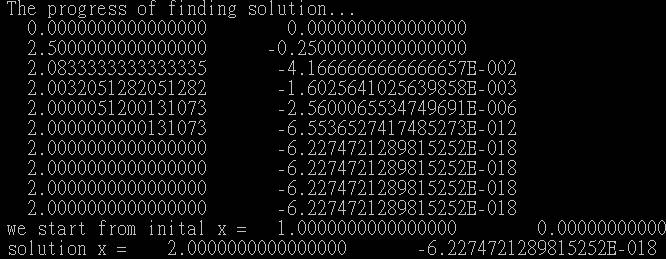
\includegraphics[scale=0.47]{pro4-3.jpg}
        \label{fig:4-2.2} 
    }
    \caption{Solution of f(x) by using n-dimension Newton's method}
    \label{fig:4-2}
\end{figure}
% %-------------------------------

% %-------------------------------
\begin{figure}[h]
    \centering
    \subfigure[N=1e8]{
        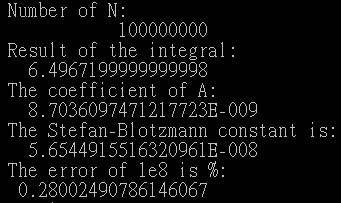
\includegraphics[scale=0.5]{pro3b8.jpg}
        \label{fig:3b-8}
    }
    \subfigure[N=1e7]{
        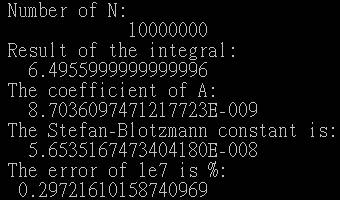
\includegraphics[scale=0.5]{pro3b7.jpg}
        \label{fig:3b-7}
    }
    \subfigure[N=1e6]{
        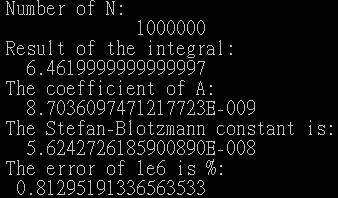
\includegraphics[scale=0.5]{pro3b6.jpg}
        \label{fig:3b-6}
    }
    \subfigure[N=1e5]{
        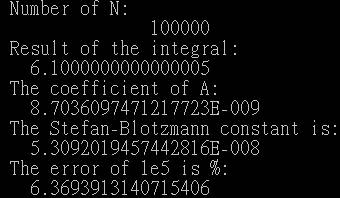
\includegraphics[scale=0.5]{pro3b5.jpg}
        \label{fig:3b-5}
    }
    \subfigure[N=1e4]{
        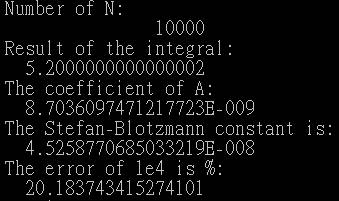
\includegraphics[scale=0.5]{pro3b4.jpg}
        \label{fig:3b-4}
    }
    \subfigure[N=1e3]{
        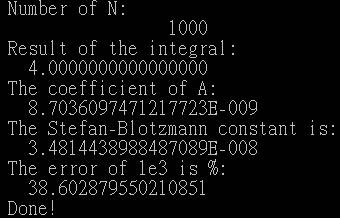
\includegraphics[scale=0.5]{pro3b3.jpg}
        \label{fig:3b-3}
    }
    \caption{Running the MC integral in different N size}
    \label{fig:3b2}
\end{figure}
% %-------------------------------

\end{document}

% \footnote{Lagrangian point:\href{https://en.wikipedia.org/wiki/Lagrange\_point}{https://en.wikipedia.org/wiki/Lagrange\_point}}


% %-------------------------------
% \begin{figure}[h]
%     \centering 
% 	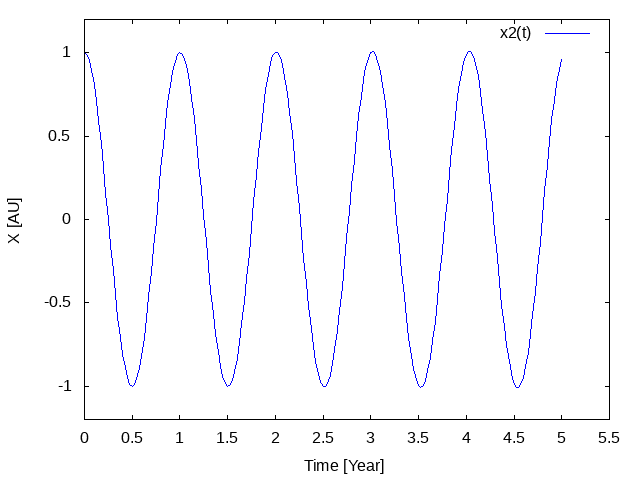
\includegraphics[scale=0.45]{pro1_x2.png}
% 	\caption{The trajectory of $m_1$ $m_2$ (when $m_2$ has a 1.25 factor of velocity).} %圖片註解
% 	\label{fig.pro1} %label 用這個就可以引用文章當中
% \end{figure}
% %-------------------------------

% %-------------------------------
% \begin{figure}[h]
%     \centering
%     \subfigure[dt=0.01yr]{
%         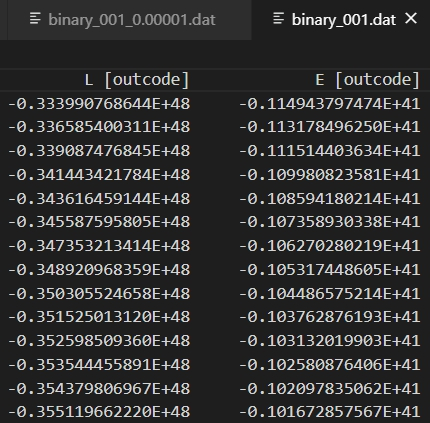
\includegraphics[scale=0.33]{01.jpg}
%         \label{01}
%     }
%     \subfigure[dt=0.001yr]{
%         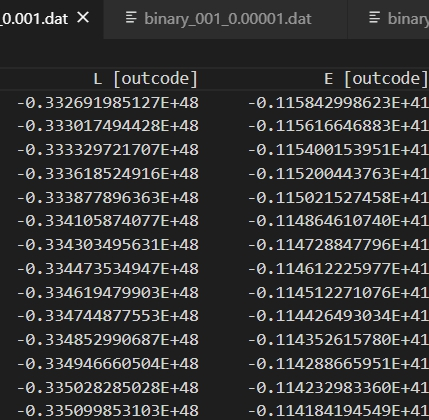
\includegraphics[scale=0.33]{001.jpg}
%         \label{001} 
%     }
%     \subfigure[dt=0.00001yr]{
%         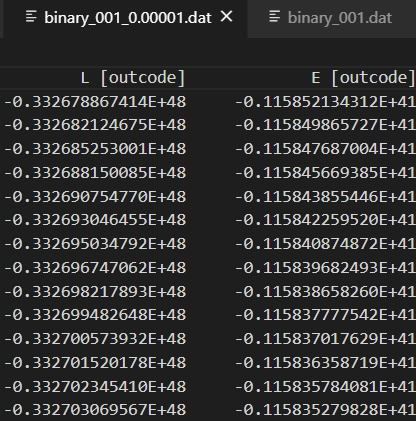
\includegraphics[scale=0.33]{00001.jpg}
%         \label{00001} 
%     }
%     \caption{L \& E in 0.01,0.001,0.00001 time step}
%     \label{fig:2c_dat}
% \end{figure}
% %-------------------------------

% \frac{\sigma ^{B}T^{4}}{\pi}=\int_{0}^{\infty }B_{\nu}(T)d\upsilon
% \quad \mbox{where} \quad
% B_{\nu}(T)=\frac{2h\upsilon ^{3}}{c^{2}}\frac{1}{e^{\frac{h\upsilon }{KT}}-1}
% \\

% set x\equiv \frac{h\upsilon }{kT}
% \upsilon =\frac{kT}{h}x
% d\upsilon =\frac{kT}{h}dx

% \\

% \Rightarrow 
% \frac{\sigma ^{B}T^{4}}{\pi}
% =
% \int_{0}^{\infty }\frac{2h\upsilon ^{3}}{c^{2}}\frac{1}{e^{\frac{h\upsilon }{KT}}-1}d\upsilon
% =\int_{0}^{\infty }\frac{2hk^3T^3}{h^3c^{2}}\frac{x^3}{e^x-1}\frac{kT}{h}dx 
% \\

% \Rightarrow 
% \sigma ^{B}=\int_{0}^{\infty }\frac{2{\pi}k^4}{h^3c^{2}}\frac{x^3}{e^x-1}dx 